%%%%%%%%%%%%%%%%%%%%%%%%%%%%%
%% Chapter 1: The template %%
%%%%%%%%%%%%%%%%%%%%%%%%%%%%%

\chapter{The template}
\label{chap:template}
This template can be used to write your thesis. The colorpalette used in this template is built around the blue of the Leiden University logo (Lei-blauw). The colors in the palette are shown in \cref{fig:template}.

\begin{figure}[!h]
	\centering
	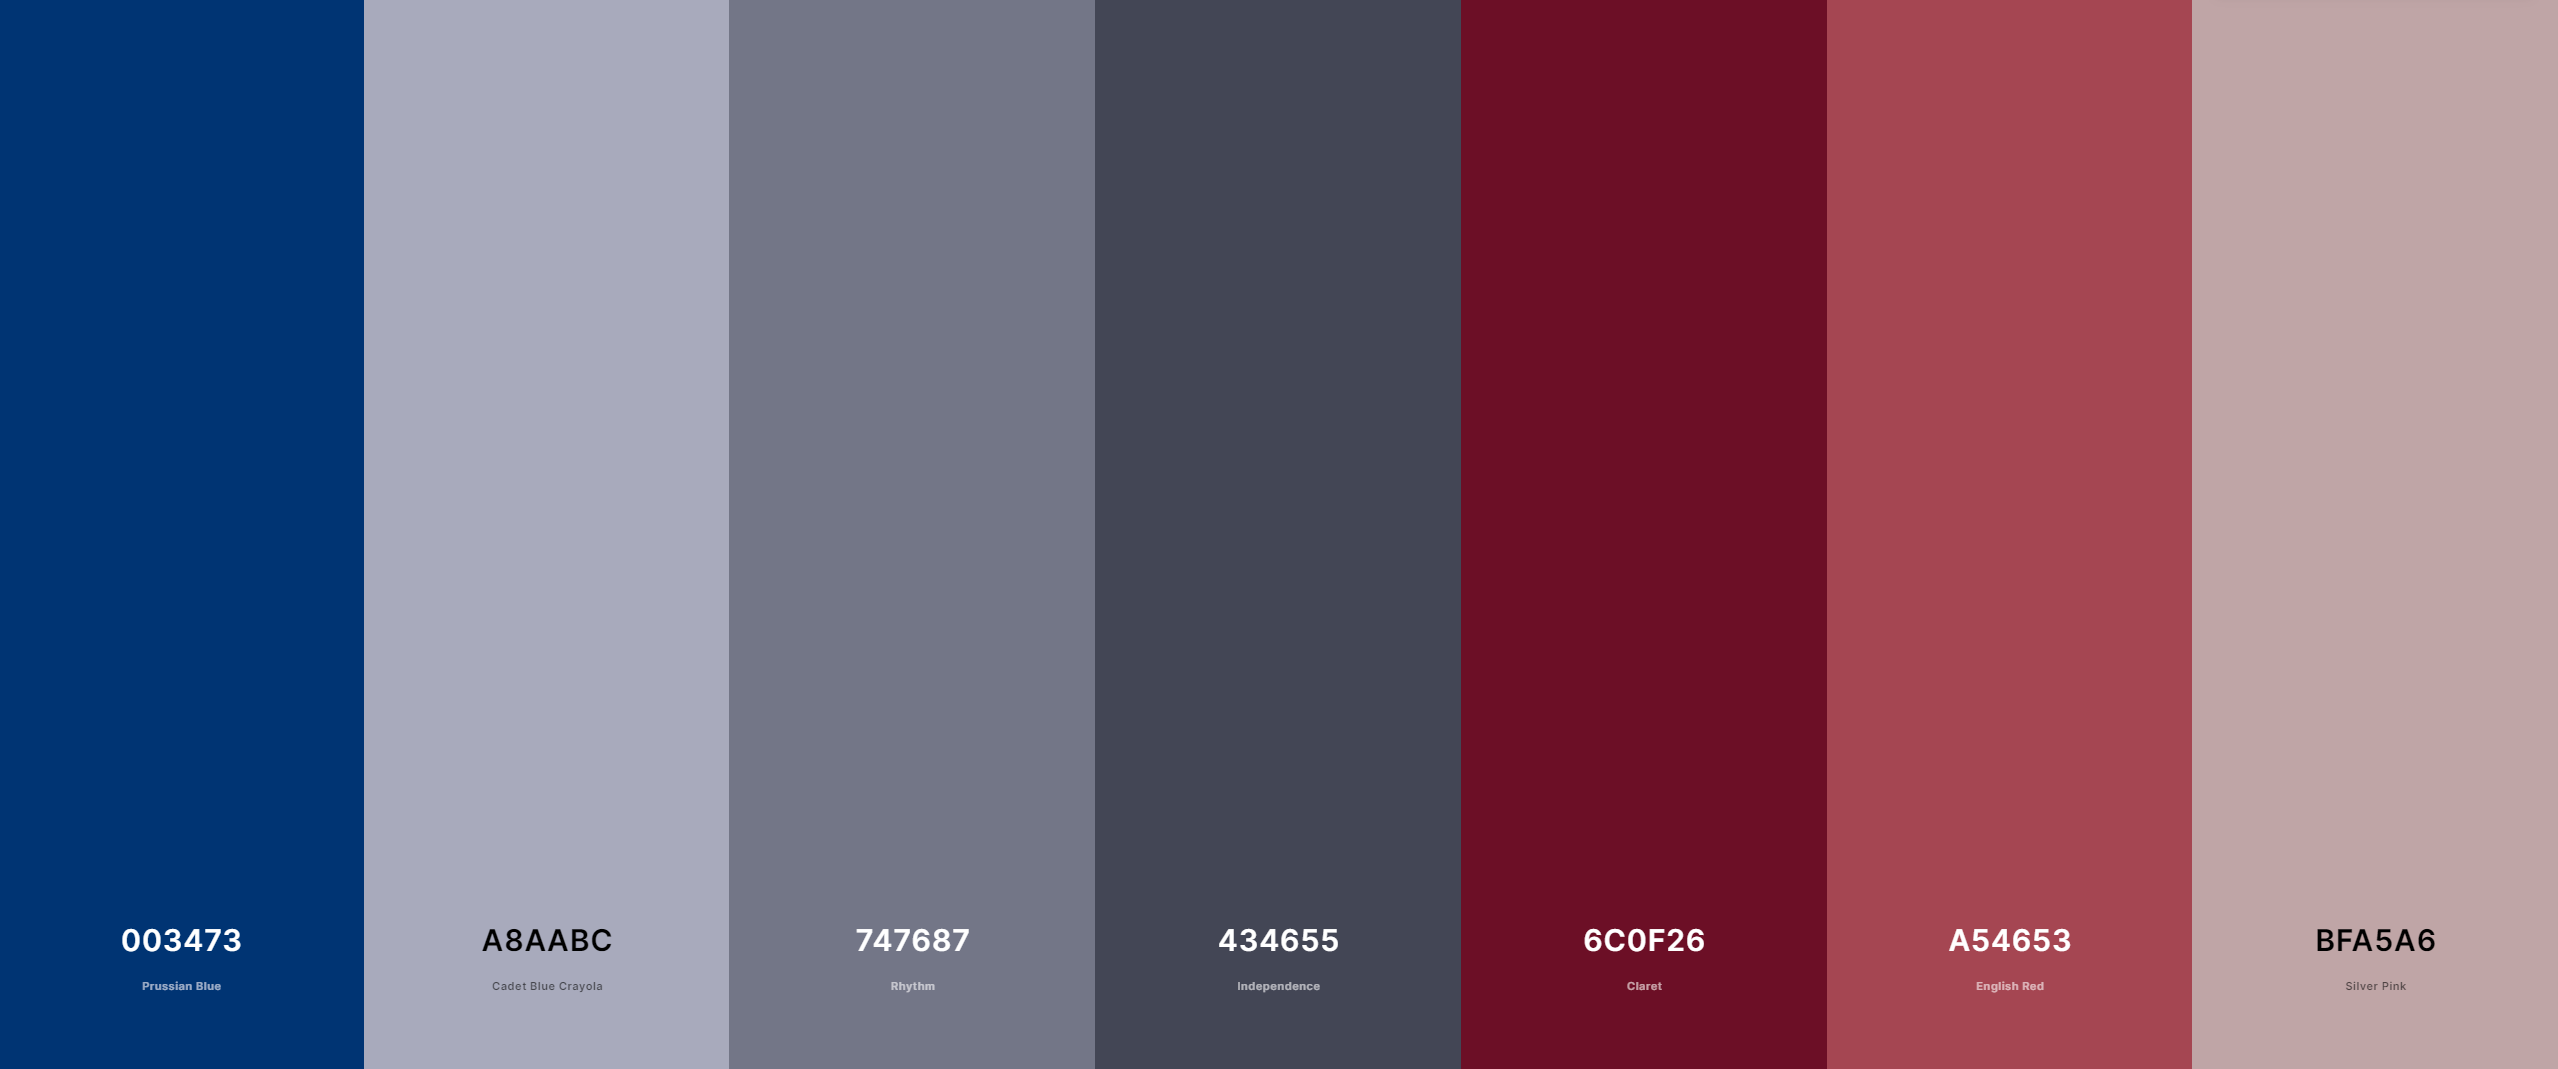
\includegraphics[width=\textwidth]{layout/figures/palette.PNG}
	\caption[Colorpalette (short caption)]{Colorpalette used in this template. Colorcodes are in hex format (HTML).}
	\label{fig:template}
\end{figure}
\noindent
\Cref{chap:tips} contains some useful tips and tricks on how to use this template and all its features. Most of these features are showcased in \cref{chap:showcase}. A Python script is included in \cref{app:script}.

